%&tekstopmaak

\documentclass[presentatie.tex]{subfiles}

%\addheadbox{section in head/foot}{\tiny\quad 1. Box}
%\addfootbox{structure}{\tiny\quad 2. Box}

%\setbeamercolor*{upper separation line head}{bg=red,fg=red}

%\makeatletter
%\setbeamertemplate{headline}
%{%
%%	\begin{beamercolorbox}{section in head/foot}
%%		\vskip2pt\insertnavigation{\paperwidth}\vskip2pt
%%		aaa
%%	\end{beamercolorbox}%
%  \begin{beamercolorbox}[colsep=1.5pt]{upper separation line head}
%\end{beamercolorbox}
%\begin{beamercolorbox}{section in head/foot}
%	\vskip2pt\insertnavigation{\paperwidth}\vskip2pt
%\end{beamercolorbox}%
%\ifbeamer@theme@subsection%
%\begin{beamercolorbox}[colsep=1.5pt]{middle separation line head}
%\end{beamercolorbox}
%\begin{beamercolorbox}[ht=2.5ex,dp=1.125ex,%
%	leftskip=.3cm,rightskip=.3cm plus1fil]{subsection in head/foot}
%	\usebeamerfont{subsection in head/foot}\insertsubsectionhead
%\end{beamercolorbox}%
%\fi%
%\begin{beamercolorbox}[colsep=1.5pt]{lower separation line head}
%\end{beamercolorbox}
%}
%\makeatother

\begin{document}
	\section{Tekstopmaak}
	\clearrecentlist
	
	%\subsection{Test}
	
	%\begin{frame}{$ \text{\LaTeX}\supset\text{Word} $}
	%	%\frametitle{$ \text{\LaTeX}\supset\text{Word} $}
	%	\begin{enumerate}
	%		\item Tekst vet / schuin
	%		\item Tekstgrootte
	%		\item Tekstkleur
	%		\item Lijntje
	%		\item Extra ruimte
	%		\item Kader
	%	\end{enumerate}
	%\end{frame}
	
	
	%\addtorecentlist{\hll|\\textbf|}
	\addtorecentlist{\textbf{\textbackslash textbf}}

	\def\extraslistsep{\hspace{0.5em}\textcolor{red!80!black}{\vrule width 1pt height 0.6\baselineskip\relax}\hspace{0.5em}}
	
	\begin{frame}<1,2,10>
		\frametitle{Teksteffecten}
		
		\renewcommand{\arraystretch}{1.5}%
		\begin{tabularx}{0.5\textwidth}{ll}
			\toprule
			Resultaat {\global\showcount=1\relax}& Code\\
			\midrule
			\showlatex{\textbf{Tekst}}{\\textbf\{Tekst\}}\\
			\showlatex{\textit{Tekst}}{\\textit\{Tekst\}}\\
			\showlatex{\textsc{Tekst}}{\\textsc\{Tekst\}}\\
			\showlatex{\underline{Tekst}}{\\underline\{Tekst\}}\\
			%\showlatex{\large{Tekst}}{\\large\{Tekst\}}\\
			\bottomrule
		\end{tabularx}%
		\begin{tabularx}{0.5\textwidth}{ll}
			\toprule
			Resultaat {\global\showcount=5\relax}& Code\\
			\midrule
			\showlatex{\texttt{Tekst}}{\\texttt\{Tekst\}}\\
			%\showlatex{\textsl{Tekst}}{\\textsl\{Tekst\}}\\
			\showlatex{{\tiny Tekst}}{\{\\tiny Tekst\}}\\
			\showlatex{{\LARGE Tekst}}{\{\\LARGE Tekst\}}\\
			{\global\showcount=9\relax}\showlatex{\textcolor{red}{Tekst}}{\\textcolor\{red\}\{Tekst\}}\only<10->{\footnote{\hll|\\usepackage\{xcolor\}|}}\\
			%\showlatex{{\Large Tekst}}{\{\\Large Tekst\}}\\
			\bottomrule
		\end{tabularx}%
		\par\addvspace{0.5\baselineskip}
		\unless\ifishandout
		%
			\only<2>{\textbf{bf} = \textbf{b}old\textbf{f}ace%
			\extraslistsep\textbf{it} = \textbf{it}alics%
			\extraslistsep\textbf{sc} = \textbf{s}mall\textbf{c}aps%
			\extraslistsep\textbf{tt} = \textbf{t}ele\textbf{t}ype (a.k.a. monospace)}%
		%
			% \only<-8>{\adjustbox{raise={-\height},set depth=20pt}{
			% 	\only<2>{\textbf{bf} = \textbf{b}old\textbf{f}ace}%
			% 	\only<3>{\textbf{it} = \textbf{it}alics}%
			% 	\only<4>{\textbf{sc} = \textbf{s}mall\textbf{c}aps}%
			% 	\only<6>{\textbf{tt} = \textbf{t}ele\textbf{t}ype (a.k.a. monospace)}
			% }}
		\fi
		\only<9->{\Huge Huge, \huge huge, \LARGE LARGE, \Large Large, \large large, \normalsize
		normalsize, \small small, \footnotesize footnotesize, \scriptsize scriptsize, \tiny tiny}
	\end{frame}

	\colorlet{curlyBrackets}{red}

	\begin{saveblock}{braces}
		\begin{highlightblock}[
			linewidth=\textwidth,gobble=12,
			framexleftmargin=0.25em,xleftmargin=0.25em
		]
			Lorem ipsum \tiny dolor sit amet, consectetur adipiscing
			elit. Phasellus elementum, lacus quis tempus
			scelerisque, elit diam vulputate ex, semper elementum
			massa odio in ante.
		\end{highlightblock}
	\end{saveblock}

	\begin{saveblock}{braces2}
		\begin{highlightblock}[
			linewidth=\textwidth,gobble=12,
			framexleftmargin=0.25em,xleftmargin=0.25em
		]
			Lorem {ipsum \tiny dolor sit ame}t, consectetur
			adipiscing elit. Phasellus {elementum}, lacus quis
			tempus scelerisque, {elit diam vulputate ex, semper}
			elementum massa odio in ante.
		\end{highlightblock}
	\end{saveblock}

	\colorlet{curlyBrackets}{red!50!blue}

	\addtorecentlist{\{\}}

	\begin{frame}
		% \begin{columns}
		% 	\begin{column}{0.5\textwidth}
		% 		\useblock{braces}
		% 	\end{column}
		% 	\begin{column}{0.5\textwidth}
		% 		\only<-1>{
		% 			\bgroup
		% 			Lorem ipsum \tiny dolor sit amet, consectetur adipiscing elit.
		% 			Phasellus elementum, lacus quis tempus scelerisque, elit diam
		% 			vulputate ex, semper elementum massa odio in ante.
		% 			\egroup
		% 		}
		% 	\end{column}
		% \end{columns}
		\adjustbox{set depth=0.4\textheight-\height}{%
			\unless\ifishandout
				\only<1>{%
					\useblock{braces}%
				}%
			\fi
			\only<2->{%
				\useblock{braces2}%
			}%
		}

		\medskip

		\adjustbox{set depth=0.4\textheight-\height}{%
			\parbox{\linewidth}{%
				\unless\ifishandout
				\only<-1>{%
					\bgroup
						Lorem ipsum \tiny dolor sit amet, consectetur adipiscing
						elit. Phasellus elementum, lacus quis tempus
						scelerisque, elit diam vulputate ex, semper elementum
						massa odio in ante.
					\egroup
				}%
				\fi
				\only<2->{%
					Lorem {ipsum \tiny dolor sit ame}t, consectetur adipiscing
					elit. Phasellus {elementum}, lacus quis tempus
					scelerisque, {elit diam vulputate ex, semper} elementum
					massa odio in ante.
				}%
			}
		}
	\end{frame}

%	\updatehighlight{
%		name=accentB,
%		add={\\, gaat}
%	}

	\begin{saveblock}{paragraphs}
		\begin{highlightblock}[linewidth=0.5\textwidth,gobble=12]
			Hallo!
			Hoe gaat het? 
		\end{highlightblock}
	\end{saveblock}

	\begin{saveblock}{paragraphs2}
		\begin{highlightblock}[linewidth=0.5\textwidth,gobble=12]
			Hallo!\\
			Hoe gaat het? 
		\end{highlightblock}
	\end{saveblock}

	% \addtorecentlist{\textbf{\textbackslash\textbackslash}}

	% \begin{frame}
	% 	\frametitle{Alinea's en regels}
		
	% 	\begin{columns}
	% 		\begin{column}{0.5\textwidth}
	% 			\useblock{paragraphs}
	% 		\end{column}
	% 		\begin{column}{0.5\textwidth}
	% 			\only<2->{
	% 				\begin{bluebox}
	% 					\setlength{\parindent}{15pt}
	% 					Hallo!
	% 					Hoe gaat het?
	% 				\end{bluebox}
	% 			}
	% 		\end{column}
	% 	\end{columns}
	
	% 	\pause
	% 	\pause
		
	% 	\medskip
	% 	Nieuwe regel in je code? Wordt genegeerd. Een nieuwe regel kan je forceren met \hll|\\\\|.
	% 	\medskip
	
	% 	\pause
	
	% 	\begin{columns}
	% 		\begin{column}{0.5\textwidth}
	% 			\useblock{paragraphs2}
	% 		\end{column}
	% 		\begin{column}{0.5\textwidth}
	% 			\only<5->{
	% 				\bgroup
	% 				%\setlength{\parskip}{6pt}
	% 				\begin{bluebox}
	% 					\setlength{\parindent}{15pt}
	% 					Hallo!\\
	% 					Hoe gaat het?
	% 				\end{bluebox}
	% 				\egroup
	% 			}
	% 		\end{column}
	% 	\end{columns}
	
	% 	\pause
	% 	\pause
		
	% 	Huh?
	% \end{frame}

	\begin{saveblock}{paragraphs}
		\begin{highlightblock}[linewidth=0.5\textwidth,gobble=12]
			Lorem ipsum dolor sit amet,
			... ornare sit amet.
			In ipsum ante, sollicitudin
			... sit amet augue.
		\end{highlightblock}
	\end{saveblock}

	\begin{saveblock}{paragraphs2}
		\begin{highlightblock}[linewidth=0.5\textwidth,gobble=12]
			Lorem ipsum dolor sit amet,
			... ornare sit amet.
			
			In ipsum ante, sollicitudin
			... sit amet augue.
		\end{highlightblock}
	\end{saveblock}

	\addtorecentlist{\textbf{witregel}}

	\begin{frame}
		\frametitle{Alinea's}
		
		\begin{columns}
			\begin{column}{0.5\textwidth}
				\useblock{paragraphs}
			\end{column}
			\begin{column}{0.5\textwidth}
				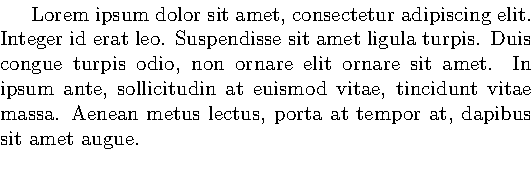
\includegraphics[width=\linewidth,height=0.5\textheight,keepaspectratio]{assets/singleParagraph2.pdf}
			\end{column}
		\end{columns}
		\pause
		\begin{columns}
			\begin{column}{0.5\textwidth}
				\useblock{paragraphs2}
			\end{column}
			\begin{column}{0.5\textwidth}
				\only<3->{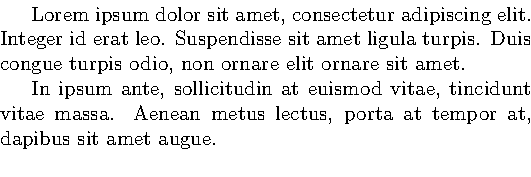
\includegraphics[width=\linewidth,height=0.5\textheight,keepaspectratio]{assets/doubleParagraph.pdf}}
			\end{column}
		\end{columns}
		\pause
	\end{frame}

	\begin{saveblock}{paragraphs}
		\begin{highlightblock}[linewidth=0.5\textwidth,gobble=12]
			...
			\usepackage{parskip}
			\begin{document}			
			Lorem ipsum dolor sit amet,
			... ornare sit amet.
			
			In ipsum ante, sollicitudin
			... sit amet augue.
			\end{document}
		\end{highlightblock}
	\end{saveblock}

	\addtorecentlist{\textbf{parskip}}

	\begin{frame}
		\frametitle{Alinea's}
		
		\begin{columns}
			\begin{column}{0.5\textwidth}
				\useblock{paragraphs}
			\end{column}
			\begin{column}{0.5\textwidth}
				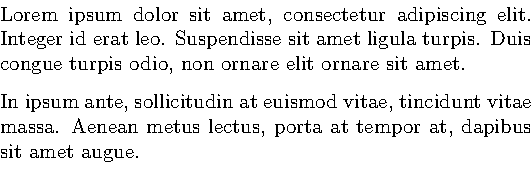
\includegraphics[width=\linewidth,height=0.8\textheight,keepaspectratio]{assets/paragraphsParskip.pdf}
				
%				\only<2->{\scriptsize{Zonder parskip:}
%				
%				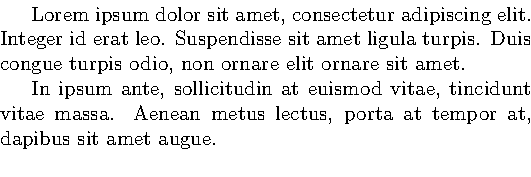
\includegraphics[width=\linewidth,height=0.5\textheight,keepaspectratio]{assets/doubleParagraph.pdf}}
			\end{column}
		\end{columns}
	\end{frame}

	\begin{saveblock}{paragraphs}
		\begin{highlightblock}[linewidth=0.5\textwidth,gobble=12]
			\noindent Lorem ipsum dolor
			sit amet, ... ornare sit
			amet.
			
			In ipsum ante, sollicitudin
			... sit amet augue.
		\end{highlightblock}
	\end{saveblock}

	\addtorecentlist{\textbf{\textbackslash noindent}}

	\begin{frame}
		\frametitle{Alinea's}
		
		\begin{columns}
			\begin{column}{0.5\textwidth}
				\useblock{paragraphs}
			\end{column}
			\begin{column}{0.5\textwidth}
				\only<2->{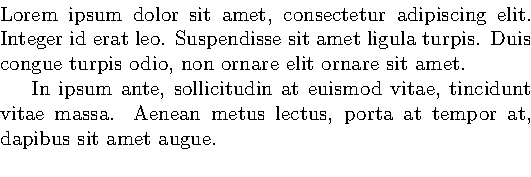
\includegraphics[width=\linewidth,height=0.5\textheight,keepaspectratio]{assets/paragraphsNoIndent.pdf}}
			\end{column}
		\end{columns}
	\end{frame}


	\begin{saveblock}{paragraphs}
		\begin{highlightblock}[linewidth=0.5\textwidth,gobble=12]
			Lorem ipsum dolor sit amet,
			... ornare sit amet.
			\vspace{1cm}
			
			In ipsum ante, sollicitudin
			... sit amet augue.
		\end{highlightblock}
	\end{saveblock}

	\addtorecentlist{\textbf{\textbackslash vspace}}
	
	\begin{frame}
		\frametitle{Alinea's}
		
		\begin{columns}
			\begin{column}{0.5\textwidth}
				\useblock{paragraphs}
			\end{column}
			\begin{column}{0.5\textwidth}
				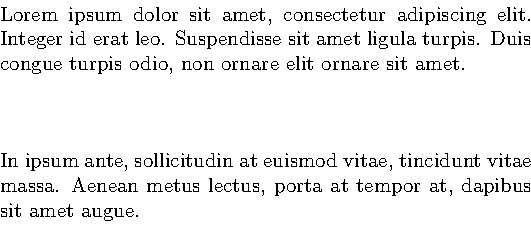
\includegraphics[width=\linewidth,height=0.8\textheight,keepaspectratio]{assets/paragraphsVspace.pdf}
			\end{column}
		\end{columns}
	
		\par\tiny{(Steeds parskip vanaf nu)}
	
	\end{frame}

	
%	\begin{frame}
%		\frametitle{Alinea's en regels}
%		
%
%	\end{frame}
	
	%\begin{frame}
	%	\frametitle{Teksteffecten}
	%	
	%	\hll|\{\\fontsize\{50\}\{60\}\\selectfont Hi!\}|
	%	\par\addvspace{10px}
	%	
	%	{\centering {\fontsize{150}{130}\selectfont Hi!}}
	%\end{frame}
	
	\addtorecentlist{\textbf{enumerate}}
	
	\begin{saveblock}{list}
		\begin{highlightblock}[linewidth=0.5\textwidth,gobble=12]
			Dit zijn de ingredi~\"e~nten:
			\begin{enumerate}
				\item Wortels
				\item Uien
				
				Lipsum dolor sit amet.
				\item Aardappelen
			\end{enumerate}
		\end{highlightblock}
	\end{saveblock}
	
	\begin{frame}
		\frametitle{Lijsten}
		
		\begin{columns}
			\begin{column}{0.5\textwidth}
				\useblock{list}
			\end{column}
			\begin{column}{0.5\textwidth}
				%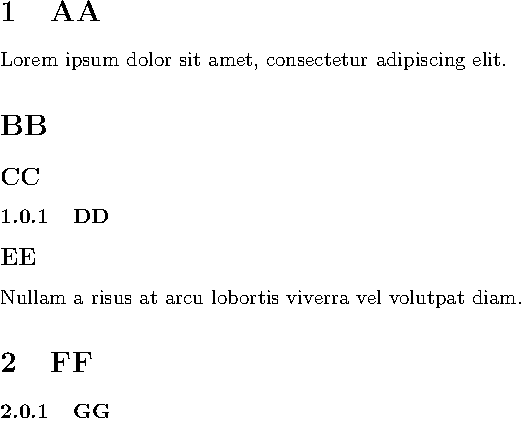
\includegraphics[width=\linewidth,height=0.8\textheight,keepaspectratio]{assets/partialNumberedStars.pdf}
				% Dit zijn de ingrediënten:
				% \begin{enumerate}
				% 	\item Wortels
				% 	\item Uien
					
				% 	Lipsum dolor sit amet.
				% 	\item Aardappelen
				% \end{enumerate}
				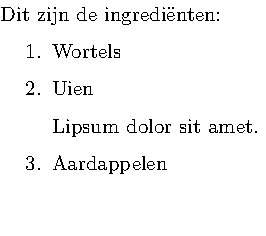
\includegraphics[width=\linewidth,height=0.8\textheight,keepaspectratio]{assets/2_Tekstopmaak/lijstEnum.pdf}
			\end{column}
		\end{columns}
	\end{frame}

	\begin{saveblock}{list}
		\begin{highlightblock}[linewidth=0.5\textwidth,gobble=12]
			Dit zijn de ingredi~\"e~nten:
			\begin{enumerate}
				\item Wortels
				\begin{enumerate}
					\item Kopen
					\item Raspen
					\item Fijnsnijden
				\end{enumerate}			
				\item Uien
				
				Lipsum dolor sit amet.
				\item Aardappelen
			\end{enumerate}
		\end{highlightblock}
	\end{saveblock}
	
	\begin{frame}
		\frametitle{Lijsten}
		
		\begin{columns}
			\begin{column}{0.5\textwidth}
				\useblock{list}
			\end{column}
			\begin{column}{0.5\textwidth}
				%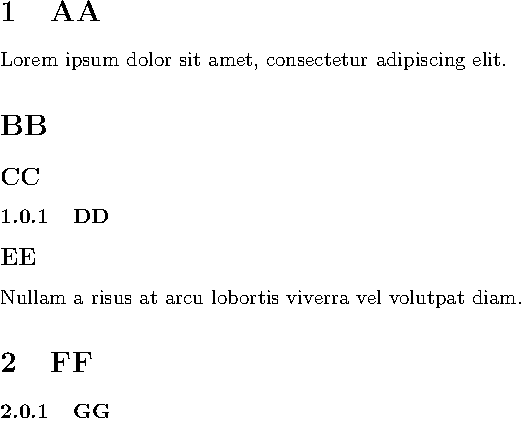
\includegraphics[width=\linewidth,height=0.8\textheight,keepaspectratio]{assets/partialNumberedStars.pdf}
				% Dit zijn de ingrediënten:
				% \begin{enumerate}
				% 	\item Wortels
				% 	\begin{enumerate}
				% 		\item Kopen
				% 		\item Raspen
				% 		\item Fijnsnijden
				% 	\end{enumerate}
				% 	\item Uien
					
				% 	Lipsum dolor sit amet.
				% 	\item Aardappelen
				% \end{enumerate}
				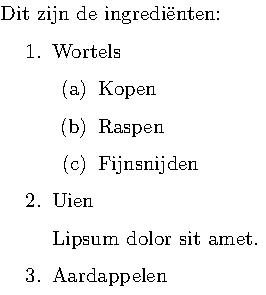
\includegraphics[width=\linewidth,height=0.8\textheight,keepaspectratio]{assets/2_Tekstopmaak/lijstEnumEnum.pdf}
			\end{column}
		\end{columns}
	\end{frame}

	\addtorecentlist{\textbf{itemize}}

	\begin{saveblock}{list}
		\begin{highlightblock}[linewidth=0.5\textwidth,gobble=12]
			Dit zijn de ingredi~\"e~nten:
			\begin{itemize}
				\item Wortels
				\begin{enumerate}
					\item Kopen
					\item Raspen
					\item Fijnsnijden
				\end{enumerate}			
				\item Uien
				
				Lipsum dolor sit amet.
				\item Aardappelen
			\end{itemize}
		\end{highlightblock}
	\end{saveblock}
	
	\begin{frame}
		\frametitle{Lijsten}
		
		\begin{columns}
			\begin{column}{0.5\textwidth}
				\useblock{list}
			\end{column}
			\begin{column}{0.5\textwidth}
				%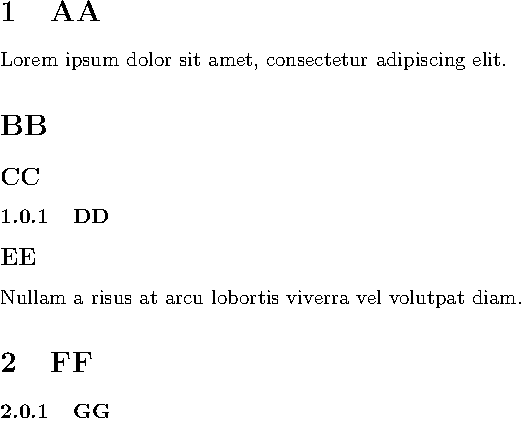
\includegraphics[width=\linewidth,height=0.8\textheight,keepaspectratio]{assets/partialNumberedStars.pdf}
				% Dit zijn de ingrediënten:
				% \begin{itemize}
				% 	\item Wortels
				% 	\begin{enumerate}
				% 		\item Kopen
				% 		\item Raspen
				% 		\item Fijnsnijden
				% 	\end{enumerate}
				% 	\item Uien
					
				% 	Lipsum dolor sit amet.
				% 	\item Aardappelen
				% \end{itemize}
				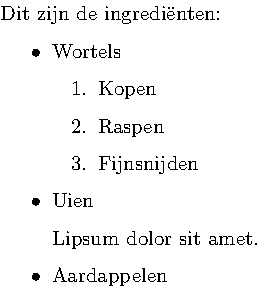
\includegraphics[width=\linewidth,height=0.8\textheight,keepaspectratio]{assets/2_Tekstopmaak/lijstItemEnum.pdf}
			\end{column}
		\end{columns}
	\end{frame}

	\begin{saveblock}{list}
		\begin{highlightblock}[linewidth=0.5\textwidth,gobble=12]
			Dit zijn de ingredi~\"e~nten:
			\begin{itemize}
				\item Wortels
				\begin{itemize}
					\item Kopen
					\item Raspen
					\item Fijnsnijden
				\end{itemize}			
				\item Uien
				
				Lipsum dolor sit amet.
				\item Aardappelen
			\end{itemize}
		\end{highlightblock}
	\end{saveblock}
	
	\begin{frame}
		\frametitle{Lijsten}
		
		\begin{columns}
			\begin{column}{0.5\textwidth}
				\useblock{list}
			\end{column}
			\begin{column}{0.5\textwidth}
				%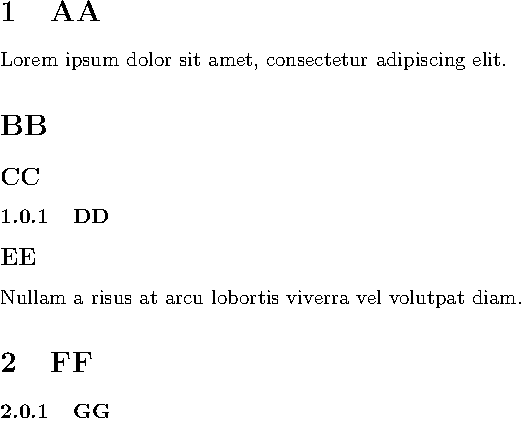
\includegraphics[width=\linewidth,height=0.8\textheight,keepaspectratio]{assets/partialNumberedStars.pdf}				
				% Dit zijn de ingrediënten:
				% \begin{itemize}
				% 	\item Wortels
				% 	\begin{itemize}
				% 		\item[\textbullet] Kopen
				% 		\item[\textbullet] Raspen
				% 		\item[\textbullet] Fijnsnijden
				% 	\end{itemize}
				% 	\item Uien
					
				% 	Lipsum dolor sit amet.
				% 	\item Aardappelen
				% \end{itemize}
				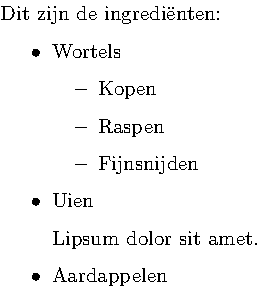
\includegraphics[width=\linewidth,height=0.8\textheight,keepaspectratio]{assets/2_Tekstopmaak/lijstItemItem.pdf}
			\end{column}
		\end{columns}
	\end{frame}

	\addtorecentlist{\textbackslash textbackslash}

	\begin{frame}
		\frametitle{Speciale tekens}

		\begingroup
		\renewcommand{\arraystretch}{1}
		\begin{tabularx}{0.45\textwidth}{ll}
			\toprule
			Code & Resultaat\\
			\midrule
			\hll|\\\{| & \{\only<2->{\hskip-10pt\relax\adjustbox{padding=-30px 0px 0px 0px,left=2ex,set height=8pt,set depth=136pt,cfbox=red 1pt,left=0pt,set depth=0pt,set height=0pt}{}}\\
			\hll|\\\}| & \}\\
			\hll|\\\%| & \%\\
			\hll|\\\_| & \_\\
			\hll|\\textasciicircum| & \textasciicircum\\
			\hll|\\\$| & \$\\
			\hll|\\textbackslash| & \textbackslash\\
			\hll|\\\&| & \&\\
			\hll|\\\#| & \#\\
			\hll|\\textgreater| & \textgreater\\
			\hll|\\textless| & \textless\\
			\bottomrule
		\end{tabularx}%
		\hfil
		\begin{tabularx}{0.5\textwidth}{ll}
			\toprule
			Code & Resultaat\\
			\midrule
			\hll|\{| & Begin groep\\
			\hll|\}| & Eindig groep\\
			\hll|\%| & Comment\\%\footnote{verschijnt niet in output}\\
			\hll|\_| & Betekenis voor wiskunde\\
			\hll|^| & Betekenis voor wiskunde\\
			\hll|\$| & Wiskundemodus\\
			\hll|\\| & Commando\\
			\hll|\&| & Kolomscheiding\\
			\hll|\#| & Parameter\\
			\hll|>| & >\\
			\hll|<| & <\\
			\bottomrule
		\end{tabularx}
		\endgroup

		% \begin{tabularx}{\textwidth}{lll}
		% 	\toprule
		% 	Resultaat {\global\showcount=1\relax}& Code & Zonder escapen\\
		% 	\midrule
		% 	\{ & \hll|\\\{| & Begin groep\\
		% 	\} & \hll|\\\}| & Eindig groep\\
		% 	\% & \hll|\\\%| & Comment: komt niet in output\\
		% 	\_ & \hll|\\\_| & Betekenis voor wiskunde\\
		% 	\^ & \hll|\\\^| & Betekenis voor wiskunde\\
		% 	\$ & \hll|\\\$| & Wiskundemodus\\
		% 	%\showlatex{\textbf{Tekst}}{\\textbf\{Tekst\}}\\
		% 	%\showlatex{\textit{Tekst}}{\\textit\{Tekst\}}\\
		% 	%\showlatex{\textsc{Tekst}}{\\textsc\{Tekst\}}\\
		% 	%\showlatex{\underline{Tekst}}{\\underline\{Tekst\}}\\
		% 	\bottomrule
		% \end{tabularx}%
	\end{frame}

	% \begin{saveblock}{specSymb}
	% 	\begin{highlightblock}[linewidth=0.5\textwidth,gobble=12]
	% 		\textbf{Hey},
	% 		\textbackslash textbf,
	% 		% Opmerking
	% 		Wel 90% {van}
	% 		de 'respondenten'
			
	% 		Wel 90\% {van}
	% 		de ~\textasciigrave~respondenten'
			
	% 		Daarom \&, \$, \{van\},
	% 		\textasciitilde,
	% 		\textasciigrave respondenten
	% 		'
	% 	\end{highlightblock}
	% \end{saveblock}

	% \addtorecentlist{\textbf{speciale tekens}}

	% \begin{frame}[t]
	% 	\frametitle{Speciale tekens}
		
	% 	\begin{onlyenv}<1>
	% 		\begin{columns}[t]
	% 			\begin{column}{0.5\textwidth}
	% 				%\raisebox{\baselineskip}{\useblock{specSymb}}
	% 				\adjustbox{valign=t}{\useblock{specSymb}}
	% 			\end{column}
	% 			\begin{column}{0.5\textwidth}
	% 				\textbf{Hey},
	% 				\textbackslash textbf,
	% 				% Opmerking
	% 				Wel 90% {van}
	% 				de 'respondenten'
	% 			\end{column}
	% 		\end{columns}
	% 	\end{onlyenv}

	% 	\begin{onlyenv}<2->
	% 		\begin{columns}
	% 			\begin{column}{0.5\textwidth}
	% 				\useblock{specSymb}
	% 			\end{column}
	% 			\begin{column}{0.5\textwidth}
	% 				\textbf{Hey},
	% 				\textbackslash textbf,
	% 				% Opmerking
	% 				Wel 90% {van}
	% 				de 'respondenten'
					
	% 				Wel 90\% {van}
	% 				de `respondenten'
					
	% 				Daarom \&, \$, \{van\},
	% 				\textasciitilde,
	% 				\textasciigrave respondenten
	% 				'

	% 				\only<3->{
	% 					\medskip
	% 					\adjustbox{scale=1.2}{
	% 					\Huge
	% 					'resp.. `resp..
	% 					}
	% 				}
	% 			\end{column}
	% 		\end{columns}
	% 	\end{onlyenv}
	% \end{frame}


	\addtorecentlist{\textasciigrave \leaders\hbox{.}\hskip 10pt\textquotesingle}

	%\def\showbig#1#2{\adjustbox{scale=3}{\adjustbox{scale=1.2}{#1}: #2}\par}
	\def\showbig#1#2{\adjustbox{scale=2.5}{\large #1: #2}\par}
	\begin{frame}{Aanhalingstekens}
		\begingroup\setlength\parskip{15pt}

		\showbig{\texttt{ \textquotesingle LaTeX\textquotesingle{} }}{'LaTeX'}
		\showbig{\texttt{ \textasciigrave LaTeX\textquotesingle{} }}{`LaTeX'}
		\showbig{\texttt{\textasciigrave\textasciigrave LaTeX\textquotesingle\textquotesingle}}{``LaTeX''}

		%\adjustbox{scale=3}{\adjustbox{scale=1.2}{\hll|'LaTeX'|}: 'LaTeX'}%\adjustbox{scale=1.2}{\Huge `LaTeX'}

		%\adjustbox{scale=3}{\adjustbox{scale=1.2}{\hll|`LaTeX'|}: `LaTeX'}

		%\hll|`LaTeX'|: \adjustbox{scale=1.2}{\Huge `LaTeX'}

		%\hll|``LaTeX''|: \adjustbox{scale=1.2}{\Huge `LaTeX'}

		%\hll|``LaTeX" ee|: \adjustbox{scale=1.2}{\Huge ``LaTeX" ee}
		\endgroup
	\end{frame}

	\begin{saveblock}{newlinewhitespace}
		\begin{highlightblock}[linewidth=0.5\textwidth,gobble=12,showspaces=true]
			Hallo ik
			ben \textellipsis.
		\end{highlightblock}
	\end{saveblock}

	\begin{saveblock}{newlinewhitespace2}
		\begin{highlightblock}[linewidth=0.5\textwidth,gobble=12,showspaces=true]
			Hallo ik%
			ben \textellipsis.
		\end{highlightblock}
	\end{saveblock}

	\setlength\atleastlength{15em}

	\begin{frame}{Spaties}

		\begin{noindentlist}
			\item<+-> \atleastwidth[\atleastlength]{\texttt{a\textvisiblespace\textvisiblespace\textvisiblespace\textvisiblespace b\textvisiblespace c}}
			a    b c.
			
			\item<+-> \leavevmode\atleastwidth[\atleastlength]{\texttt{a\hll|\\|\textvisiblespace
			\hll|\\|\textvisiblespace
			\hll|\\|\textvisiblespace
			\hll|\\|\textvisiblespace b\textvisiblespace c}}
			a\ \ \ \ b c.

			\item<+-> \atleastwidth[\atleastlength]{\hll|a\\quad b c\\,d\\;e|}
			a\quad b c\,d\;e

			\item<.-> \atleastwidth[\atleastlength]{\hll|a\\hspace\{2cm\}b|}
			a\hspace{2cm}b
			
			\item<+-> \atleastwidth[\atleastlength]{\hll|Ik kan \\LaTeX schrijven!|}
			Ik kan \LaTeX schrijven!
	
			\item<.-> \atleastwidth[\atleastlength]{\hll|Vincent is lid van de \\TeX niCie.|}
			Vincent is lid van de \TeX niCie.
	
			\item<+-> \atleastwidth[\atleastlength]{\hll|Ik kan \\LaTeX\{\}|\hll|\ schrijven!|}
			Ik kan \LaTeX{} schrijven!

			\item<+-> \adjustbox{valign=T,raise=10pt}{\atleastwidth[\textwidth/2]{\useblock{newlinewhitespace}}} Hallo ik
			ben \textellipsis.

			\item<.-> \adjustbox{valign=T,raise=10pt}{\atleastwidth[\textwidth/2]{\useblock{newlinewhitespace2}}} Hallo ik%
			ben \textellipsis.
		\end{noindentlist}
	\end{frame}

%	\begin{frame}
%		\begin{enumerate}
%			\item Speciale tekens
%			\item Lijsten
%			\item Pagina layout
%			\item Inhoudstafel
%		\end{enumerate}
%	\end{frame}
\end{document}
